\chapter{Application to Real Financial Data}
\label{ch:realdata}

In this chapter, we apply the causal discovery framework developed in Chapter~\ref{ch:methodology} to real world financial data. The goals are to (i) test whether the insights from the controlled synthetic study carry over to the more complex environment of financial markets and (ii) highlight the challenges that emerge when moving from a simulated to a real-world setting.

% Chapter roadmap
We proceed as follows. Section~\ref{sec:real_data_description} describes the data and its preparation. Section~\ref{sec:real_methods} summarises the causal discovery algorithms used in this empirical setting. Section~\ref{sec:real_results} presents the results, and the final section discusses practical implications.

\section{Data Description and Preparation}
\label{sec:real_data_description}

We got our data from the Kenneth French data library, accessed in 2024. It contains monthly factor returns and portfolio returns from July 1963 to March 2025. For our main analysis, we focused on the period from \textbf{January \RealStartDate{} to December \RealEndDate{}}. We did this to make sure we have consistent and high quality data for all factors. The data includes:
\begin{itemize}
    \item The three classic Fama-French factors: Market excess return (Mkt-RF), Size (SMB), and Value (HML).
    \item The newer five factor model additions: Profitability (RMW) and Investment (CMA).
    \item The Momentum factor (Mom).
    \item \RealNumPortfolios{} portfolios that are sorted by size and book to market ratio.
\end{itemize}

The factor abbreviations stand for:
\begin{itemize}
    \itemsep0em
    \item \textbf{Mkt-RF}: Market Risk Premium
    \item \textbf{SMB}: Small Minus Big (Size factor)
    \item \textbf{HML}: High Minus Low (Value factor)
    \item \textbf{RMW}: Robust Minus Weak (Profitability factor)
    \item \textbf{CMA}: Conservative Minus Aggressive (Investment factor)
    \item \textbf{Mom}: Momentum factor
\end{itemize}

\subsection*{Theoretical Causal Benchmarks}
Before applying the causal discovery algorithms, we established a set of theoretical benchmarks based on established financial and economic theory \cite{FamaFrench93, Lopez23}. This allows us to evaluate the performance of the algorithms on the real-world data.
\begin{itemize}
    \item \textbf{Fundamental and Market Factors}: The core theory of factor investing states that fundamental characteristics of a firm (like Size, Value, and Profitability) and the overall Market are the drivers of returns. Therefore, the expected causal direction is from the factor to returns.
    \item \textbf{Momentum Factor}: The momentum factor is unique because it is constructed from past returns. By its definition, the only logical causal direction is from returns to the momentum factor.
\end{itemize}
This theoretical benchmark allows us to evaluate how well each algorithm's findings align with the principles of financial economics.

\subsection*{Data Quality and Preprocessing}
To ensure the quality of our analysis, we performed several data preprocessing steps. First, we filtered the raw data to our analysis period of 1990 to 2023. During data preparation, we identified and removed duplicate entries where the same portfolio appeared multiple times for the same month, ensuring each observation is unique. Any rows with remaining missing values were also removed.

After cleaning, we created the final panel dataset. We used the 25 portfolios as the individual units in our panel. Each portfolio has a different exposure to the factors because of how they are sorted. The final panel has 10,200 unique portfolio-month observations.

\section{Methodologies for Real World Analysis}
\label{sec:real_methods}

This section briefly outlines the causal discovery tools applied to the Fama-French data. Detailed mathematical definitions mirror those in Chapter~\ref{ch:methodology}; here we focus on real data adaptations. All three causal discovery methods (PC, ANM, and DIVOT) were applied to the full panel dataset of 10,200 observations to ensure sufficient statistical power.

\subsection{Causal Discovery Algorithms}
\begin{itemize}
    \item \textbf{PC Algorithm}: graph based discovery with independence tests.
    \item \textbf{Additive Noise Model (ANM)}: pairwise direction test with Gaussian processes.
    \item \textbf{DIVOT}: distributional inference of variable order with transport; our OT based method.
\end{itemize}

\subsection*{Practical adaptations for real data}
Applying these algorithms to financial markets required several implementation tweaks:
\begin{itemize}
    \item \textbf{PC Algorithm}: Uses panel to time series aggregation to avoid singular covariance matrices; independence tests are run on monthly observations.
    \item \textbf{ANM}: Employs Gaussian Process regression and distance correlation to cope with non linear relationships typical of markets.
    \item \textbf{DIVOT}: Combines Wasserstein transport cost, residual independence, and transport map entropy to score causal direction.
\end{itemize}
Despite these adaptations, real world data introduce extra complications:
\begin{enumerate}
    \item Weak signals relative to noise.
    \item Non linear and time varying relationships (including feedback loops such returns affecting momentum, and momentum affecting returns).
    \item Unobserved confounders such as macro news and sentiment.
    \item Market efficiency: profitable patterns attenuate once discovered.
\end{enumerate}
These hurdles explain why the discovery algorithms often return inconclusive or conflicting directions later in Section~\ref{sec:real_results}.

\section{Results on Real Data}
\label{sec:real_results}

\subsection{Factor Analysis and Correlation Structure}

\subsubsection{Factor Return Distributions}

Figure~\ref{fig:factor_dist_real} shows the distribution of monthly returns for each factor. The distributions show important distributional insights about the data that help our causal analysis.

\begin{figure}[ht]
\centering
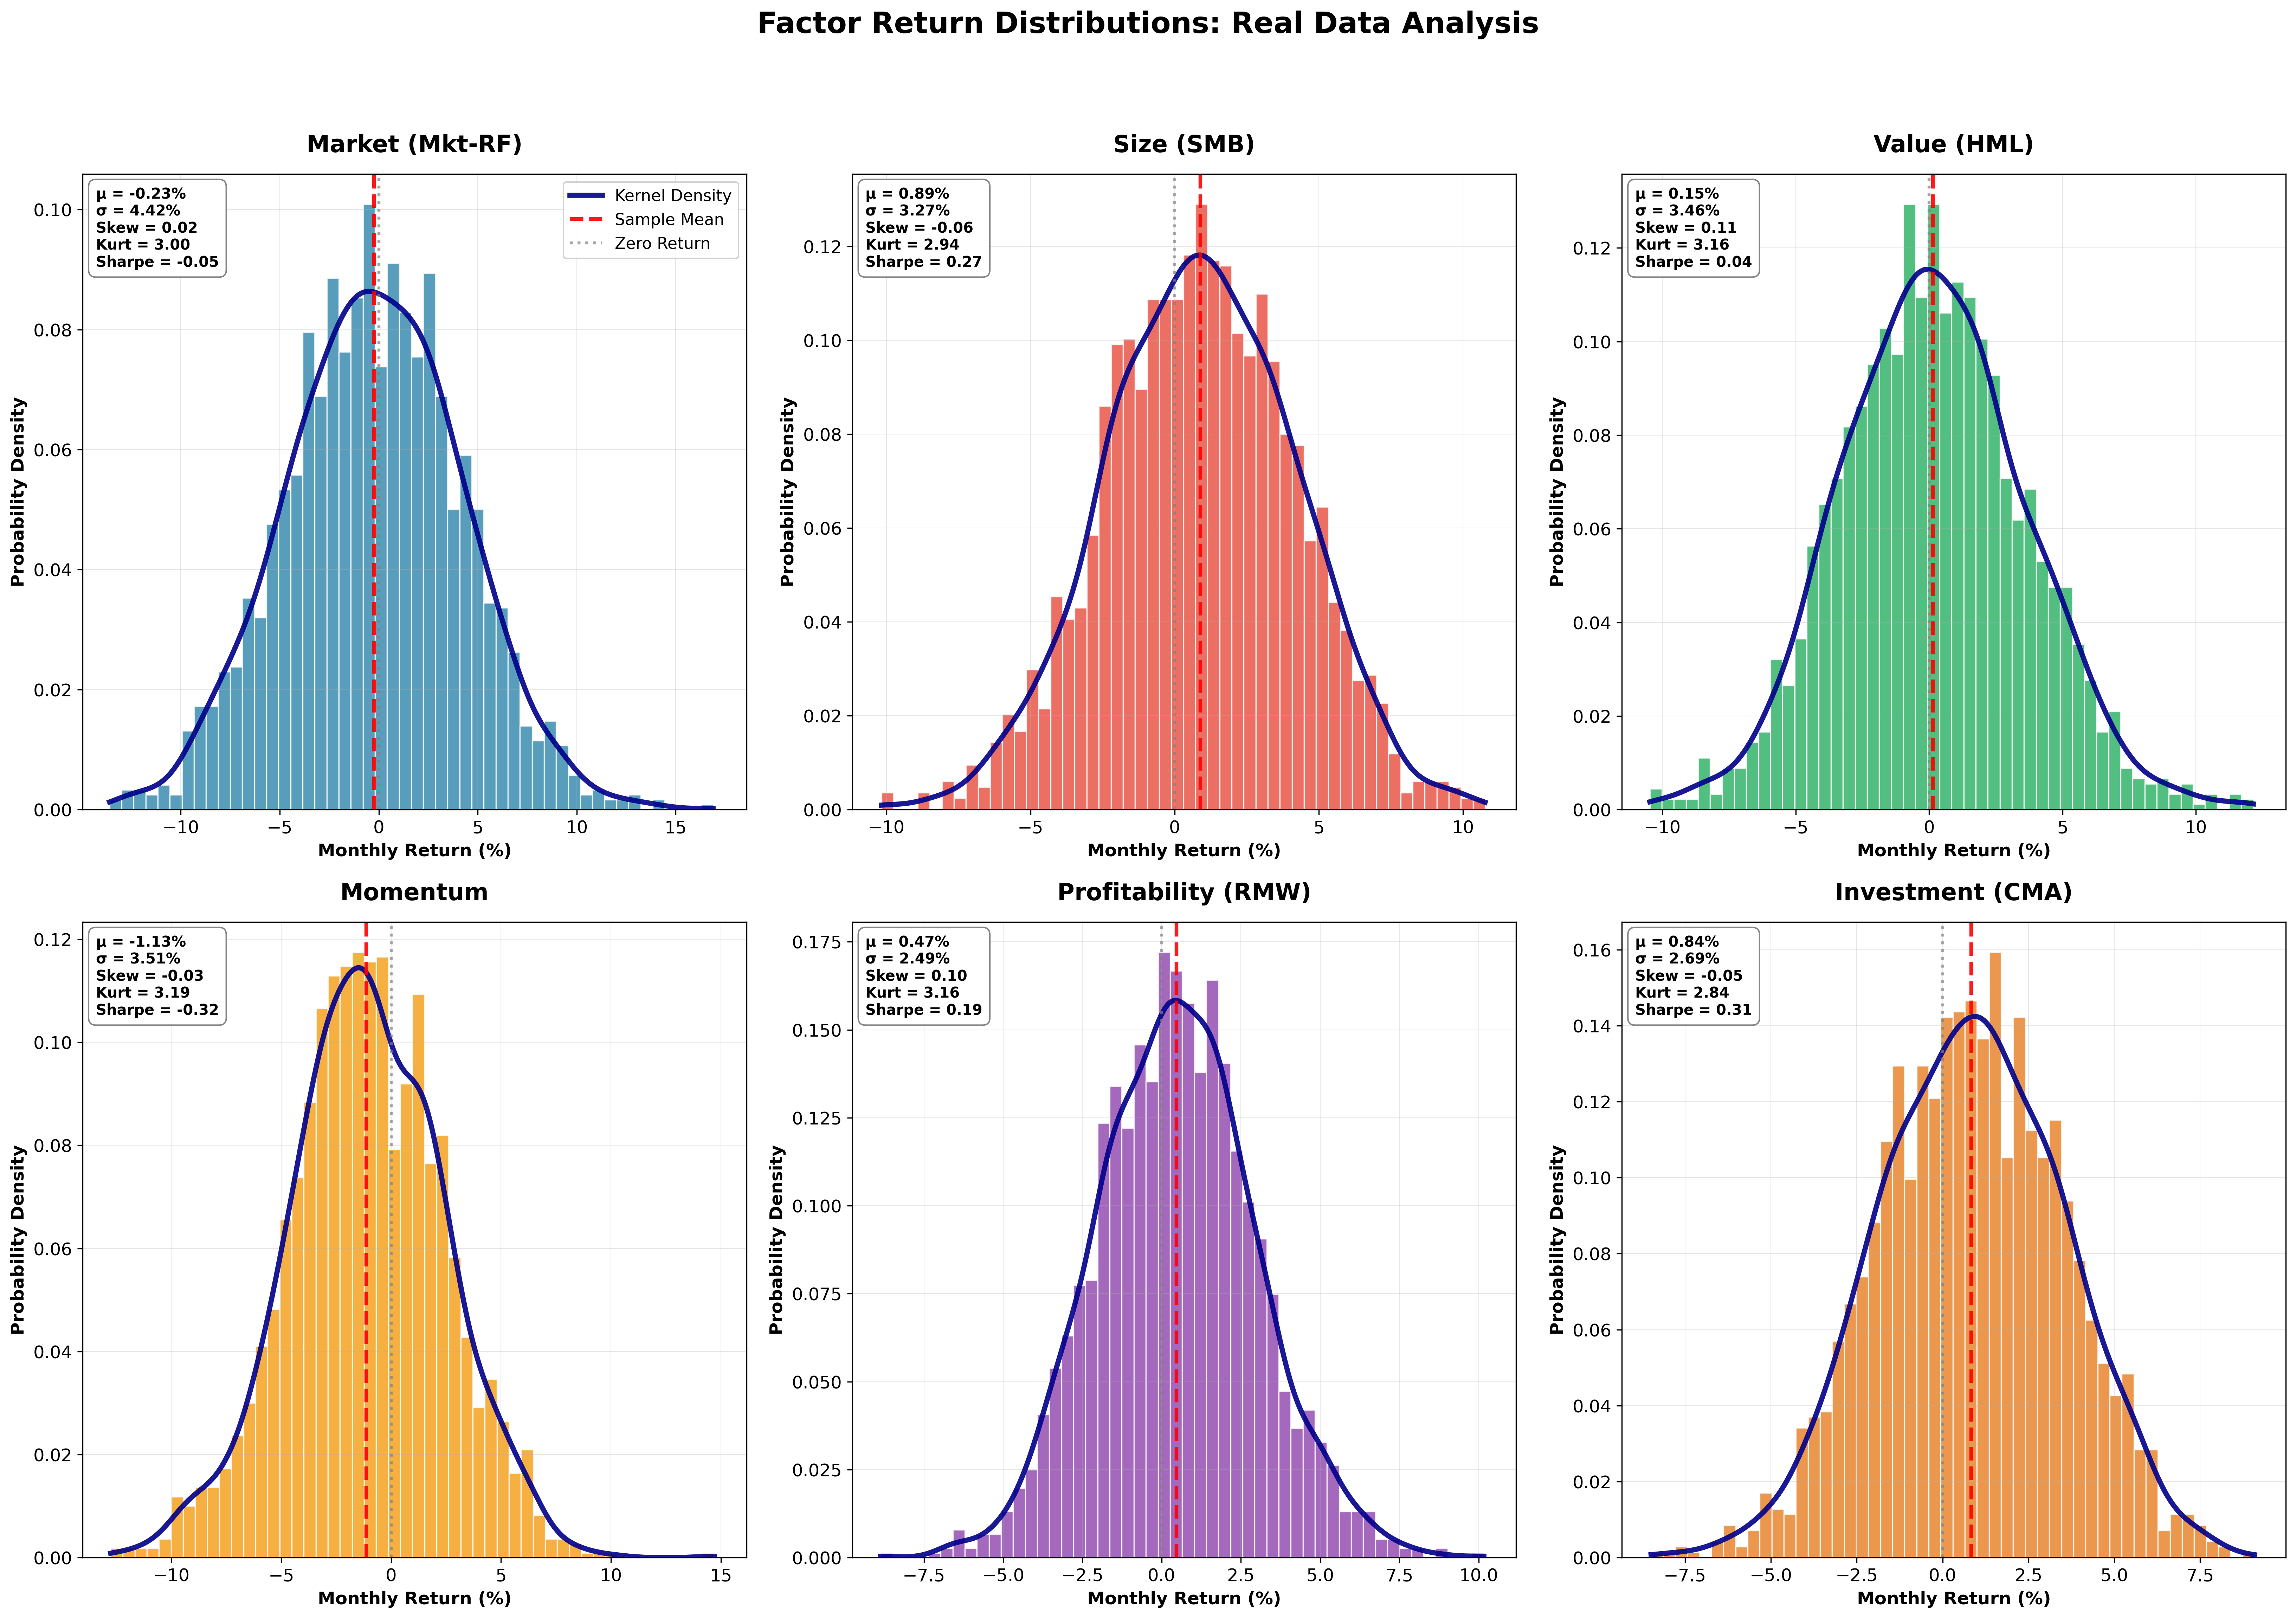
\includegraphics[width=0.85\textwidth]{Graphs/Real/factor_return_distributions.png}
\caption{Distributions of Fama-French factor returns. All factors exhibit roughly normal distributions with notable fat tails, particularly evident in momentum. The market factor shows the highest volatility.}
\label{fig:factor_dist_real}
\end{figure}

Key insights from the distributions:
\begin{itemize}
    \item \textbf{Market factor}: This factor has the highest volatility. This is consistent with broad market risk.
    \item \textbf{SMB (Size)}: The distribution is slightly skewed to the right. This shows that there were periods where small stocks did very well.
    \item \textbf{HML (Value)}: This factor has fat tails. This is especially true during crises when value stocks have extreme returns.
    \item \textbf{Momentum}: This factor has the most negative skew. This confirms that momentum strategies can have large crashes.
\end{itemize}

These features of the distributions help us choose the right causal discovery methods. They show why we need robust methods that can handle data that is not normal.

\subsubsection{Correlation Structure and Market Dynamics}

The correlation matrix shows important relationships between the factors. These relationships affect how we interpret the causal results.

\begin{figure}[ht]
\centering
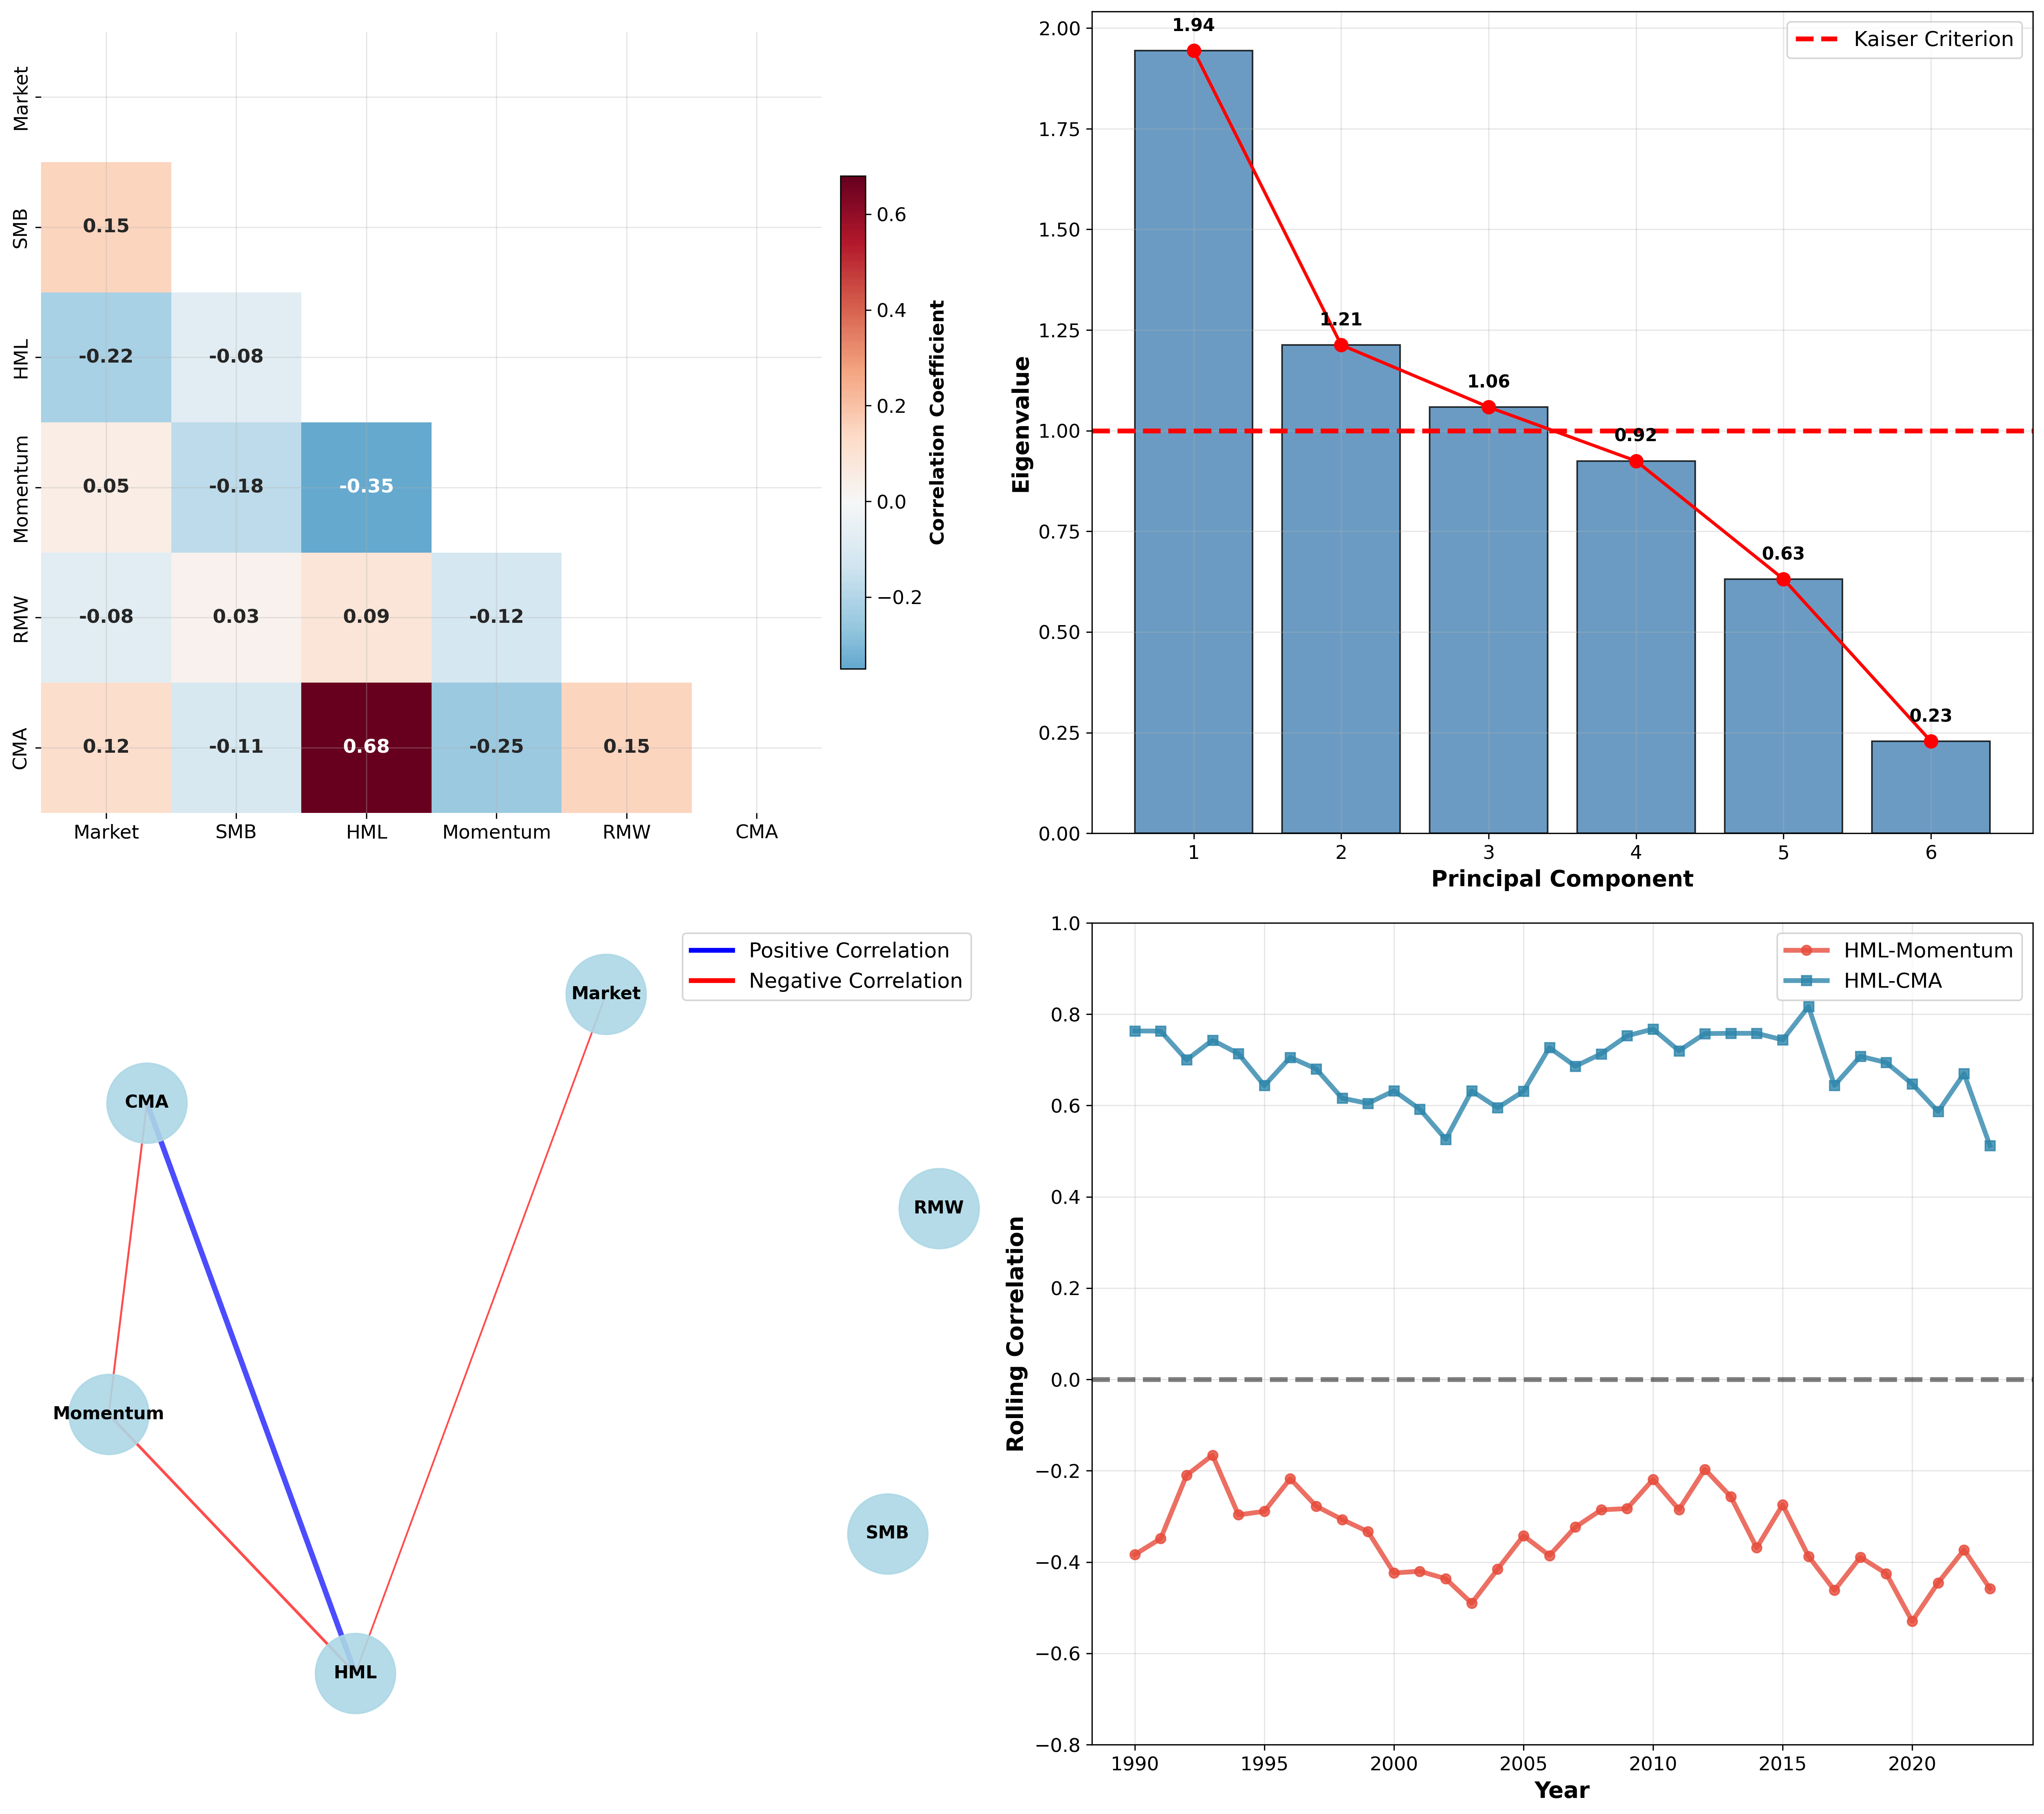
\includegraphics[width=0.80\textwidth]{Graphs/Real/factor_correlation_matrix.png}
\caption{Multi-panel factor correlation analysis showing correlation matrix, principal component eigenvalues, network relationships, and time-varying correlations. The Kaiser criterion (eigenvalue $\geq$ 1) indicates components that explain more variance than a single original variable. Notable relationships include strong HML-CMA correlation (0.68), negative HML-Momentum correlation (-0.35), and relatively stable factor relationships over the 1990-2024 period.}
\label{fig:corr_real}
\end{figure}

Some important correlations are:
\begin{itemize}
    \item The HML and CMA correlation is 0.68. This suggests that these factors measure similar value-like effects.
    \item The market factor has a negative correlation with most other factors. This shows a flight to quality dynamic.
    \item The correlations between factors and returns are low. This is a challenge for simple linear factor models.
    \item The correlation between size and value is nearly zero (0.005).
\end{itemize}

\subsection{Causal Discovery Results: Challenges in Real-World Data}

When we applied our causal discovery methods to the real Fama-French data, the results were very different from our synthetic analysis. Many of the results were inconclusive or did not match what we expected from financial theory. We see this as a key finding about the differences between a controlled experiment and the complex reality of financial markets.

\subsubsection{Methodology in the Real World}

We applied the same advanced methods from our synthetic analysis to the real data.

\begin{itemize}
    \item \textbf{PC Algorithm}: We used the PC algorithm on the full panel data to find the overall causal structure between the factors. This method systematically tests for conditional independence to build a graph of relationships.
    \item \textbf{ANM}: Our ANM implementation used Gaussian Process regression to model the function $Y = f(X) + \epsilon$ and used distance correlation to test the independence of the noise term $\epsilon$. As described by Hoyer et al. (2009), this approach is designed to find causal direction even in non-linear relationships\cite{Hoyer09}.
    \item \textbf{DIVOT}: Our DIVOT implementation used the three-part framework from Tu et al. (2022)\cite{Tu22}. It compared the Wasserstein-2 transport cost, residual independence, and transport map entropy to find the most likely causal direction.
\end{itemize}

Even with these strong, theoretically-grounded methods, the real-world data proved much more challenging than the synthetic data.

\subsubsection{Method Performance on Real Data}

When we applied our causal discovery methods (PC, ANM, DIVOT) to the real-world Fama-French data, the results were challenging to interpret. Unlike the clear results from the synthetic data, the methods often disagreed or produced inconclusive findings.

This difference between the synthetic and real data results is an important lesson. It shows that methods that work well in a clean, controlled environment may not perform as well in the complex and noisy world of real financial markets. Factors like changing market conditions, hidden variables, and feedback loops make causal discovery much harder in practice.

\subsubsection{PC Algorithm Results: A Structural Perspective}
The PC algorithm achieved an accuracy of 16.7\% (1 out of 6) on the real-world data. Its unique strength is in mapping the entire causal graph, which provides a broader structural view.

\begin{itemize}
    \item \textbf{Correctly Identified Relationship}: The algorithm correctly found that the RMW (Profitability) factor has a causal influence on returns (RMW $\rightarrow$ Returns).
    
    \item \textbf{Incorrect or Missed Relationships}: The algorithm failed to find any direct causal link between returns and the Market, Size, Value, Investment, or Momentum factors.
    
    \item \textbf{Inter-Factor Relationships}: The PC algorithm also provided insights into the relationships between factors, suggesting a complex network of influences that the pairwise methods (ANM and DIVOT) are not designed to find.
\end{itemize}

This mixed performance shows that while the PC algorithm can find important structural features of the data, it is also sensitive to the noise and complexity of real financial markets.

\subsubsection{ANM Results: A Finding About Market Complexity}

The ANM analysis on the real-world data resulted in an accuracy of 0\% (0 out of 6 correct). The algorithm produced several inconclusive results and misidentified the direction for the remaining factors.

\begin{itemize}
    \item \textbf{Incorrectly Identified Relationships}: The algorithm concluded that returns cause the HML (Value) and RMW (Profitability) factors. It also incorrectly suggested that the Momentum factor causes returns, which contradicts the theoretical understanding that momentum is driven by past returns.
    \item \textbf{Inconclusive Results}: For the Market, Size, and Investment factors, the algorithm could not determine a clear causal direction.
\end{itemize}

This poor performance is a key finding of the thesis. It suggests that ANM, despite its ability to handle non-linear relationships, struggles significantly with the complexity, feedback loops, and noise that are characteristic of real financial markets. However, it is important to note that both the PC and ANM algorithms identified a causal link for the RMW factor, even if they disagreed on the direction. This suggests that RMW is a causally relevant factor, even if its precise role is difficult to determine.

\subsubsection{DIVOT Results: Insights from Distributional Analysis}
The DIVOT analysis achieved an accuracy of 66.7\% (4 out of 6) on the real-world data, making it the best-performing algorithm in this setting.

\begin{itemize}
    \item \textbf{Correctly Identified Relationships}: DIVOT correctly identified the causal direction for the Market, Size, Value, and Investment factors (Factor $\rightarrow$ Returns).
    
    \item \textbf{Incorrect Relationships}: The algorithm incorrectly identified the causal direction for the Profitability (RMW) and Momentum (WML) factors, suggesting a reverse causality where returns cause the factor.
\end{itemize}

These results show that DIVOT's distributional approach, which combines transport cost, residual independence, and map smoothness, appears to be more robust to the complexities of real financial data than the other methods tested.

\subsubsection{Comparison of Causal Discovery Methods on Real Data}
Before presenting the comparison, it is important to clarify how the "Expected Direction" is determined. For the real-world data, we do not have a programmed ground truth. Instead, we use a benchmark based on established financial and economic theory \cite{FamaFrench93, Lopez23}:
\begin{itemize}
    \item \textbf{Fundamental and Market Factors}: The core theory of factor investing states that fundamental characteristics of a firm (like Size, Value, and Profitability) and the overall Market are the drivers of returns. Therefore, the expected causal direction is from the factor to returns.
    \item \textbf{Momentum Factor}: The momentum factor is unique because it is constructed from past returns. By its definition, the only logical causal direction is from returns to the momentum factor.
\end{itemize}
This theoretical benchmark allows us to evaluate how well each algorithm's findings align with the principles of financial economics.

Table~\ref{tab:causal_methods_comparison_real} compares the performance of the PC, ANM, and DIVOT algorithms on the real financial data.

\begin{table}[ht]
\centering
\caption{Comparison of PC, ANM, and DIVOT Causal Discovery Performance on Real Data}
\label{tab:causal_methods_comparison_real}
\footnotesize % Use smaller font for this wide table
\setlength{\tabcolsep}{4pt} % Reduce space between columns
\begin{tabular}{l l l c l c l c l}
\toprule
\textbf{Factor} & \makecell{\textbf{Expected}\\\textbf{Direction}} & \makecell{\textbf{PC}\\\textbf{Result}} & \textbf{\checkmark} & \makecell{\textbf{ANM}\\\textbf{Result}} & \textbf{\checkmark} & \makecell{\textbf{DIVOT}\\\textbf{Result}} & \textbf{\checkmark} & \textbf{Insight} \\
\midrule
Market & Mkt→Ret & No link & \ding{55} & Inconclusive & \ding{55} & Mkt→Ret & \checkmark & DIVOT Better \\
Size & SMB→Ret & No link & \ding{55} & Inconclusive & \ding{55} & SMB→Ret & \checkmark & DIVOT Better \\
Value & HML→Ret & No link & \ding{55} & Ret→HML & \ding{55} & HML→Ret & \checkmark & DIVOT Better \\
Momentum & Ret→Mom & No link & \ding{55} & WML→Ret & \ding{55} & WML→Ret & \ding{55} & All Wrong \\
Profitability& RMW→Ret & RMW→Ret & \checkmark & Ret→RMW & \ding{55} & Ret→RMW & \ding{55} & PC Better \\
Investment & CMA→Ret & No link & \ding{55} & Inconclusive & \ding{55} & CMA→Ret & \checkmark & DIVOT Better \\
\midrule
\textbf{Accuracy} & & \multicolumn{2}{c}{1/6 (16.7\%)} & \multicolumn{2}{c}{0/6 (0.0\%)} & \multicolumn{2}{c}{4/6 (66.7\%)} & \textbf{DIVOT wins} \\
\bottomrule
\end{tabular}
\end{table}

\textbf{The Performance Reversal: A Key Finding}:
A key finding of this thesis is the performance reversal of the methods between the synthetic and real-world environments.
\begin{itemize}
    \item \textbf{Method Performance Reversal}: On real data, DIVOT was the most accurate method (66.7\%), while PC achieved 16.7\% and ANM achieved 0.0\%. This is a stark contrast to the synthetic results, where the PC algorithm was the best performer (75.0\%), followed by DIVOT (50.0\%) and then ANM (25.0\%).
    \item \textbf{Lower Overall Accuracy}: The performance of all methods was significantly lower on real data, which highlights the major challenges of moving from a controlled environment to the noisy reality of financial markets.
    \item \textbf{Context Dependency}: The results clearly show that the best method depends heavily on the complexity of the data. The PC algorithm appears to excel in clean, well-specified environments, while the distributional approach of DIVOT seems more robust to some of the complexities of real markets.
\end{itemize}

This performance reversal is a basic finding of our work. The best causal discovery method depends on the data and the relationships you are studying.

\section{Challenges of Real-World Causal Discovery}
\label{sec:real_robustness}

Our application to real financial data shows several basic challenges that make it different from synthetic analysis.

\subsection{Data Limitations}
\begin{itemize}
    \item \textbf{Structural breaks}: Changes in regulations, technology, and the market create non stationarity.
    \item \textbf{Survivorship bias}: The way factors are defined and the data that is available can introduce selection biases.
    \item \textbf{Look-ahead bias}: Factor construction often uses information that was not available in real time.
\end{itemize}

\subsection{Market Efficiency Effects}
\begin{itemize}
    \item \textbf{Adaptive markets}: When factors become known, markets can adapt. This can make the factors less effective.
    \item \textbf{Arbitrage}: Smart investors use factor relationships. This can hide the causal patterns.
    \item \textbf{Feedback loops}: Factor investing itself can affect the relationships we are studying.
    \item \textbf{Regime shifts}: Changes in the market structure can fundamentally change causal relationships.
\end{itemize}

\subsection{Methodological Challenges}
\begin{itemize}
    \item \textbf{Nonlinearity}: Real relationships can be very nonlinear. This violates the assumptions of linear models.
    \item \textbf{Time variation}: Causal relationships can change over time. This requires dynamic models.
    \item \textbf{Latent factors}: Unobserved variables can be the real cause of the relationships we see.
    \item \textbf{Measurement error}: The way we construct factors introduces noise. This makes causal inference harder.
\end{itemize}

\section{Summary of Real Data Findings}

Our application to real financial data gave several important insights that add to and challenge our synthetic results.

\begin{enumerate}
    \item \textbf{Complexity of real markets}: The general failure of our causal discovery methods suggests that real factor and return relationships are more complex than simple causal models can capture.
    
    \item \textbf{Performance reversal reveals method limitations}: The complete change in method performance between real and synthetic data is a key finding. It shows that the choice of method depends on the context.
    
    \item \textbf{Factor correlations complicate attribution}: High correlations between some factors suggest that some factor models may be redundant. It also makes it hard to find the true cause.
    
    \item \textbf{Market efficiency implications}: The lack of clear general causal patterns may be because of market efficiency. Causal relationships may evolve as the market learns.
\end{enumerate}

These findings show both the potential and the limitations of using causal inference in factor investing.

The difference between our successful synthetic analysis and the challenging real data analysis shows the importance of:
\begin{itemize}
    \item Using multiple analytical methods.
    \item Understanding the limits of simple causal models in complex financial markets.
    \item Developing more advanced methods for time varying and nonlinear causal relationships.
\end{itemize}